% =====================================================================
% ARTIGO — Projeto de Banco de Dados (Unidade II) — Tema 07: Oficina Mecânica
% Formato SBC (mesma formatação do modelo-tcc-sbc.tex fornecido)
% Compilar:  pdflatex artigo-oficina-sbc.tex  (duas vezes)
% =====================================================================
\documentclass[a4paper,12pt]{article}

\usepackage[utf8]{inputenc}
\usepackage[T1]{fontenc}
\usepackage[brazilian]{babel}
\usepackage{times}
\usepackage[a4paper,top=3.5cm,left=3cm,right=3cm,bottom=2.5cm]{geometry}
\usepackage{graphicx}
\usepackage{url}
\usepackage{indentfirst}
\usepackage{titlesec}
\usepackage[bf,sf,footnotesize,indent]{caption}
\usepackage{longtable}
\usepackage{array}

\setlength{\parindent}{1.27cm}
\setlength{\parskip}{6pt}
\flushbottom

\titleformat{\section}{\fontsize{13}{15}\bfseries}{\thesection.}{1em}{}
\titleformat{\subsection}{\fontsize{12}{14}\bfseries}{\thesubsection.}{1em}{}
\titleformat{\subsubsection}{\fontsize{12}{14}\bfseries\itshape}{\thesubsubsection.}{1em}{}
\titlespacing*{\section}{0pt}{12pt}{6pt}
\titlespacing*{\subsection}{0pt}{10pt}{4pt}

\renewcommand{\captionfont}{\sffamily\footnotesize\bfseries}
\setlength{\captionmargin}{0.8cm}
\captionsetup{labelsep=period}

\newenvironment{resumo}{%
  \list{}{\advance\topsep by6pt\relax
    \leftmargin=0.8cm
    \labelwidth=0pt
    \listparindent=0pt
    \itemindent\listparindent
    \rightmargin\leftmargin}\item[\hskip\labelsep\bfseries\itshape Resumo.]\itshape}%
  {\endlist}

\renewenvironment{abstract}{%
  \list{}{\advance\topsep by6pt\relax
    \leftmargin=0.8cm
    \labelwidth=0pt
    \listparindent=0pt
    \itemindent\listparindent
    \rightmargin\leftmargin}\item[\hskip\labelsep\bfseries\itshape Abstract.]\itshape}%
  {\endlist}

\newcommand{\cod}[1]{\texttt{\small #1}}

\begin{document}
\pagestyle{empty}
\sloppy

\begin{center}
  {\fontsize{16}{20}\selectfont\bfseries Integridade e Desempenho no Controle de Ordens de Serviço de uma Oficina Mecânica: Restrições, Gatilhos e Índices Verificados por Testes em PostgreSQL}\\[4pt]
  {\fontsize{14}{18}\selectfont\bfseries Integrity and Performance in Work Order Management for an Auto Repair Shop: Constraints, Triggers and Indexes Verified by Tests in PostgreSQL}\\[12pt]

  {\normalsize\bfseries Jarlisson Brito Santos$^{1}$, Brunno Passos$^{1}$, Caio Vinicius$^{1}$}\\[4pt]
  {\footnotesize\itshape Professor(a): [Nome do(a) Professor(a)] -- Disciplina: Banco de Dados}\\[6pt]

  {\normalsize
    $^{1}$[Curso] — Universidade Tiradentes (UNIT)\\{}
    Aracaju, Sergipe -- SE\\{}
    \footnotesize\texttt{britojarlisson64@gmail.com, brunnopassos1@gmail.com, caiovinicius200361@gmail.com}
  }
\end{center}
\vspace{12pt}

\begin{resumo}
Oficinas mecânicas de pequeno e médio porte costumam controlar ordens de
serviço em papel ou planilhas, o que permite placas duplicadas, peças
aplicadas sem baixa no estoque, ordens sem mecânico responsável e ordens
já fechadas sendo alteradas. Este trabalho modela e implementa em
PostgreSQL 16 um banco de dados para esse cenário, com seis tabelas,
domínios de formato, restrições declarativas, cinco regras de negócio
em gatilhos e oito índices, cada um ligado a uma consulta real. Toda
decisão foi verificada por teste executado: 34 casos de tipos,
restrições e regras foram automatizados e todos tiveram o resultado
esperado, comparado pelo código SQLSTATE devolvido pelo banco. Sobre uma
base sintética de 300 mil ordens de serviço, os índices reduziram a
consulta do histórico por placa de 30,60~ms para 0,25~ms e as páginas
lidas de 8.323 para 31, com custo de 26\% a mais na inserção em lote. Os
testes também mostraram limites: um índice sobre coluna de baixa
seletividade foi ignorado pelo otimizador, e uma visão reescrita com
\emph{LATERAL} foi 633 vezes mais rápida em consultas seletivas, mas
duas vezes mais lenta em relatórios que varrem a tabela inteira. Conclui-se
que levar as regras para o banco elimina as falhas descritas e que cada
índice precisa ser justificado por medição, e não por suposição.
\end{resumo}
\noindent\textbf{Palavras-chave:} banco de dados relacional, integridade de dados, gatilhos, índices, PostgreSQL.

\vspace{6pt}

\begin{abstract}
Small and medium-sized auto repair shops often track work orders on
paper or spreadsheets, which allows duplicate license plates, parts used
without stock deduction, orders with no responsible mechanic and closed
orders being changed. This work models and implements a PostgreSQL 16
database for this scenario, with six tables, format domains, declarative
constraints, five business rules in triggers and eight indexes, each
tied to a real query. Every design decision was verified by an executed
test: 34 type, constraint and rule cases were automated and all of them
produced the expected outcome, checked against the SQLSTATE code
returned by the database. On a synthetic dataset of 300,000 work orders,
the indexes reduced the plate history query from 30.60~ms to 0.25~ms and
the pages read from 8,323 to 31, at a cost of 26\% slower bulk inserts.
The tests also exposed limits: an index on a low-selectivity column was
ignored by the planner, and a view rewritten with \emph{LATERAL} was 633
times faster for selective queries but twice as slow for reports that
scan the whole table. We conclude that moving the rules into the
database removes the failures described and that each index must be
justified by measurement rather than assumption.
\end{abstract}
\noindent\textbf{Keywords:} relational database, data integrity, triggers, indexes, PostgreSQL.

\vspace{18pt}

% =====================================================================
\section{Introdução}

Em uma oficina mecânica, a ordem de serviço (OS) é o documento que liga
o cliente, o veículo, o mecânico que executa o serviço e as peças
aplicadas. Quando esse controle é feito em papel ou em planilhas, os
erros aparecem no balcão: o mesmo veículo é cadastrado duas vezes com a
placa digitada de formas diferentes, peças saem da prateleira sem baixa
no estoque, a OS não registra quem foi o mecânico responsável e uma OS
já paga é alterada depois, gerando divergência no faturamento. Também é
comum o hodômetro ``voltar'' por erro de digitação, o que invalida o
histórico de revisões, e a busca pelo histórico de um carro demora
enquanto o cliente espera.

Esses problemas têm um ponto em comum: as regras existem na cabeça das
pessoas, mas não em nenhum lugar que as obrigue a serem cumpridas. Um
sistema gerenciador de banco de dados relacional permite declarar essas
regras junto com os dados, de modo que nenhuma aplicação, planilha
importada ou digitação apressada consiga violá-las
\cite{codd1970,elmasri2016}.

O objetivo geral deste trabalho é projetar, implementar e verificar por
testes um banco de dados para o controle de ordens de serviço de uma
oficina mecânica. Os objetivos específicos são: (i) modelar as entidades
do problema e escolher tipos de dados adequados; (ii) implementar as
regras de negócio como restrições e gatilhos; (iii) criar índices
orientados às consultas da oficina e medir o efeito de cada um; e (iv)
documentar cada afirmação com um teste executado e sua evidência, em um
repositório no GitHub acompanhado por uma metodologia ágil.

O restante do texto está organizado assim: a Seção~2 apresenta a
fundamentação; a Seção~3 descreve a metodologia; a Seção~4 mostra a
arquitetura, as decisões e os resultados dos testes; e a Seção~5 traz as
conclusões.

% =====================================================================
\section{Fundamentação e Trabalhos Relacionados}

O modelo relacional representa os dados em relações e garante a
consistência por meio de chaves e restrições de integridade
\cite{codd1970}. Na prática, os SGBDs oferecem integridade de entidade
(\emph{PRIMARY KEY}), integridade referencial (\emph{FOREIGN KEY}, com
ações como \emph{RESTRICT} e \emph{CASCADE}), unicidade (\emph{UNIQUE}),
obrigatoriedade (\emph{NOT NULL}) e regras de domínio (\emph{CHECK})
\cite{elmasri2016,silberschatz2019}. Regras que dependem de outras
tabelas ou da transição de estado de uma linha não cabem em um
\emph{CHECK} e são implementadas com gatilhos (\emph{triggers})
\cite{silberschatz2019,pgdocs}.

No PostgreSQL, além dos tipos nativos, é possível criar domínios
(\emph{CREATE DOMAIN}), que reúnem um tipo base e uma regra de validação
reaproveitável, e tipos enumerados (\emph{ENUM}) \cite{pgdocs}. Para o
desempenho, o índice B-tree é o padrão; índices parciais indexam apenas
as linhas que atendem a um predicado; e índices GIN com a extensão
\emph{pg\_trgm} aceleram buscas por trechos de texto (\emph{LIKE}/
\emph{ILIKE} com curinga no início) \cite{pgdocs}. Winand
\cite{winand2012} mostra que o ganho de um índice depende da
seletividade do filtro e da ordem das colunas em índices compostos, e
que todo índice tem custo na escrita, pontos que este trabalho
verificou experimentalmente. O comando \emph{EXPLAIN ANALYZE} executa a
consulta e informa o plano escolhido, o tempo real e as páginas lidas,
e foi a ferramenta usada para todas as medições \cite{pgdocs}.

Em relação aos livros-texto, que apresentam esses recursos de forma
isolada, a contribuição deste trabalho é aplicá-los a um problema
concreto e, principalmente, tratar cada decisão como uma hipótese a ser
testada, incluindo os casos em que o recurso \emph{não} trouxe o efeito
esperado.

% =====================================================================
\section{Metodologia}

\textbf{Ambiente.} Os testes foram executados no PostgreSQL 16.15, em
Linux (Ubuntu 24.04), com o cliente \emph{psql}. Os scripts de
automação foram escritos em Python 3 e chamam o \emph{psql}, de modo
que qualquer pessoa reproduz o experimento com o comando
\cod{./scripts/rodar\_tudo.sh}. O mesmo script é executado pelo GitHub
Actions a cada envio ao repositório, com um contêiner PostgreSQL 16.

\textbf{Dados.} Para que o efeito dos índices fosse mensurável, foi
gerada uma base sintética e determinística (\cod{setseed}) com 20.000
clientes, 30.000 veículos, 25 mecânicos (3 inativos), 500 peças,
300.000 ordens de serviço entre 2021 e outubro de 2026 e 450.435 itens
de peça. O volume equivale a cerca de seis anos de uma rede de oficinas
e foi aumentado de propósito: com poucas centenas de linhas, qualquer
consulta é rápida e os índices não fazem diferença. Por ser uma carga
histórica, os gatilhos de regra foram desligados apenas durante a
carga, mas as chaves estrangeiras permaneceram ativas.

\textbf{Testes de tipos, restrições e regras.} Cada caso de teste é um
arquivo SQL com o resultado esperado declarado: ``ERRO'' acompanhado do
código SQLSTATE que o banco deve devolver (por exemplo, 23505 para
violação de unicidade) ou ``OK'', quando o comando deve ser aceito e uma
consulta final de verificação deve retornar \cod{PASSOU}. Cada teste
roda dentro de \cod{BEGIN} \dots{} \cod{ROLLBACK}, para que um teste não
interfira no seguinte. Comparar o SQLSTATE, e não apenas a ocorrência de
um erro, evita aceitar como correto um teste que falhou pelo motivo
errado.

\textbf{Testes de índices.} Cada consulta foi executada com
\cod{EXPLAIN (ANALYZE, BUFFERS)} sete vezes; registrou-se a mediana do
tempo de execução, o tipo de acesso escolhido pelo otimizador e o total
de páginas lidas. A medição foi feita primeiro só com os índices
criados automaticamente por \emph{PRIMARY KEY} e \emph{UNIQUE} e depois
com os índices do arquivo \cod{sql/04\_indices.sql}, sempre após
\cod{VACUUM ANALYZE}. O custo na escrita foi medido com a inserção de
20.000 OS (mediana de três execuções, desfeitas com \cod{ROLLBACK}).

\textbf{Gestão do projeto.} O trabalho foi organizado em Scrum
simplificado com cinco sprints semanais (26/10 a 30/11/2026),
registradas como \emph{milestones} no GitHub, com o backlog em
\emph{issues} e um quadro Kanban no GitHub Projects \cite{scrum2020}. A
definição de pronto exige, para cada item, o SQL no repositório, um
teste automatizado e a evidência gerada.

% =====================================================================
\section{Desenvolvimento e Resultados}

\subsection{Arquitetura e modelo de dados}

A Figura~\ref{fig:der} apresenta o modelo. O cliente possui veículos; o
veículo recebe ordens de serviço; cada OS tem exatamente um mecânico
responsável; e a relação N:N entre OS e peças é resolvida pela tabela
associativa \cod{os\_peca}, cuja chave primária é composta por
\cod{(id\_os, id\_peca)}. A tabela guarda o \cod{preco\_unitario}
copiado da peça no momento do lançamento: se o preço do catálogo mudar
depois, o valor das OS antigas não muda.

\begin{figure}[!htbp]
  \centering
  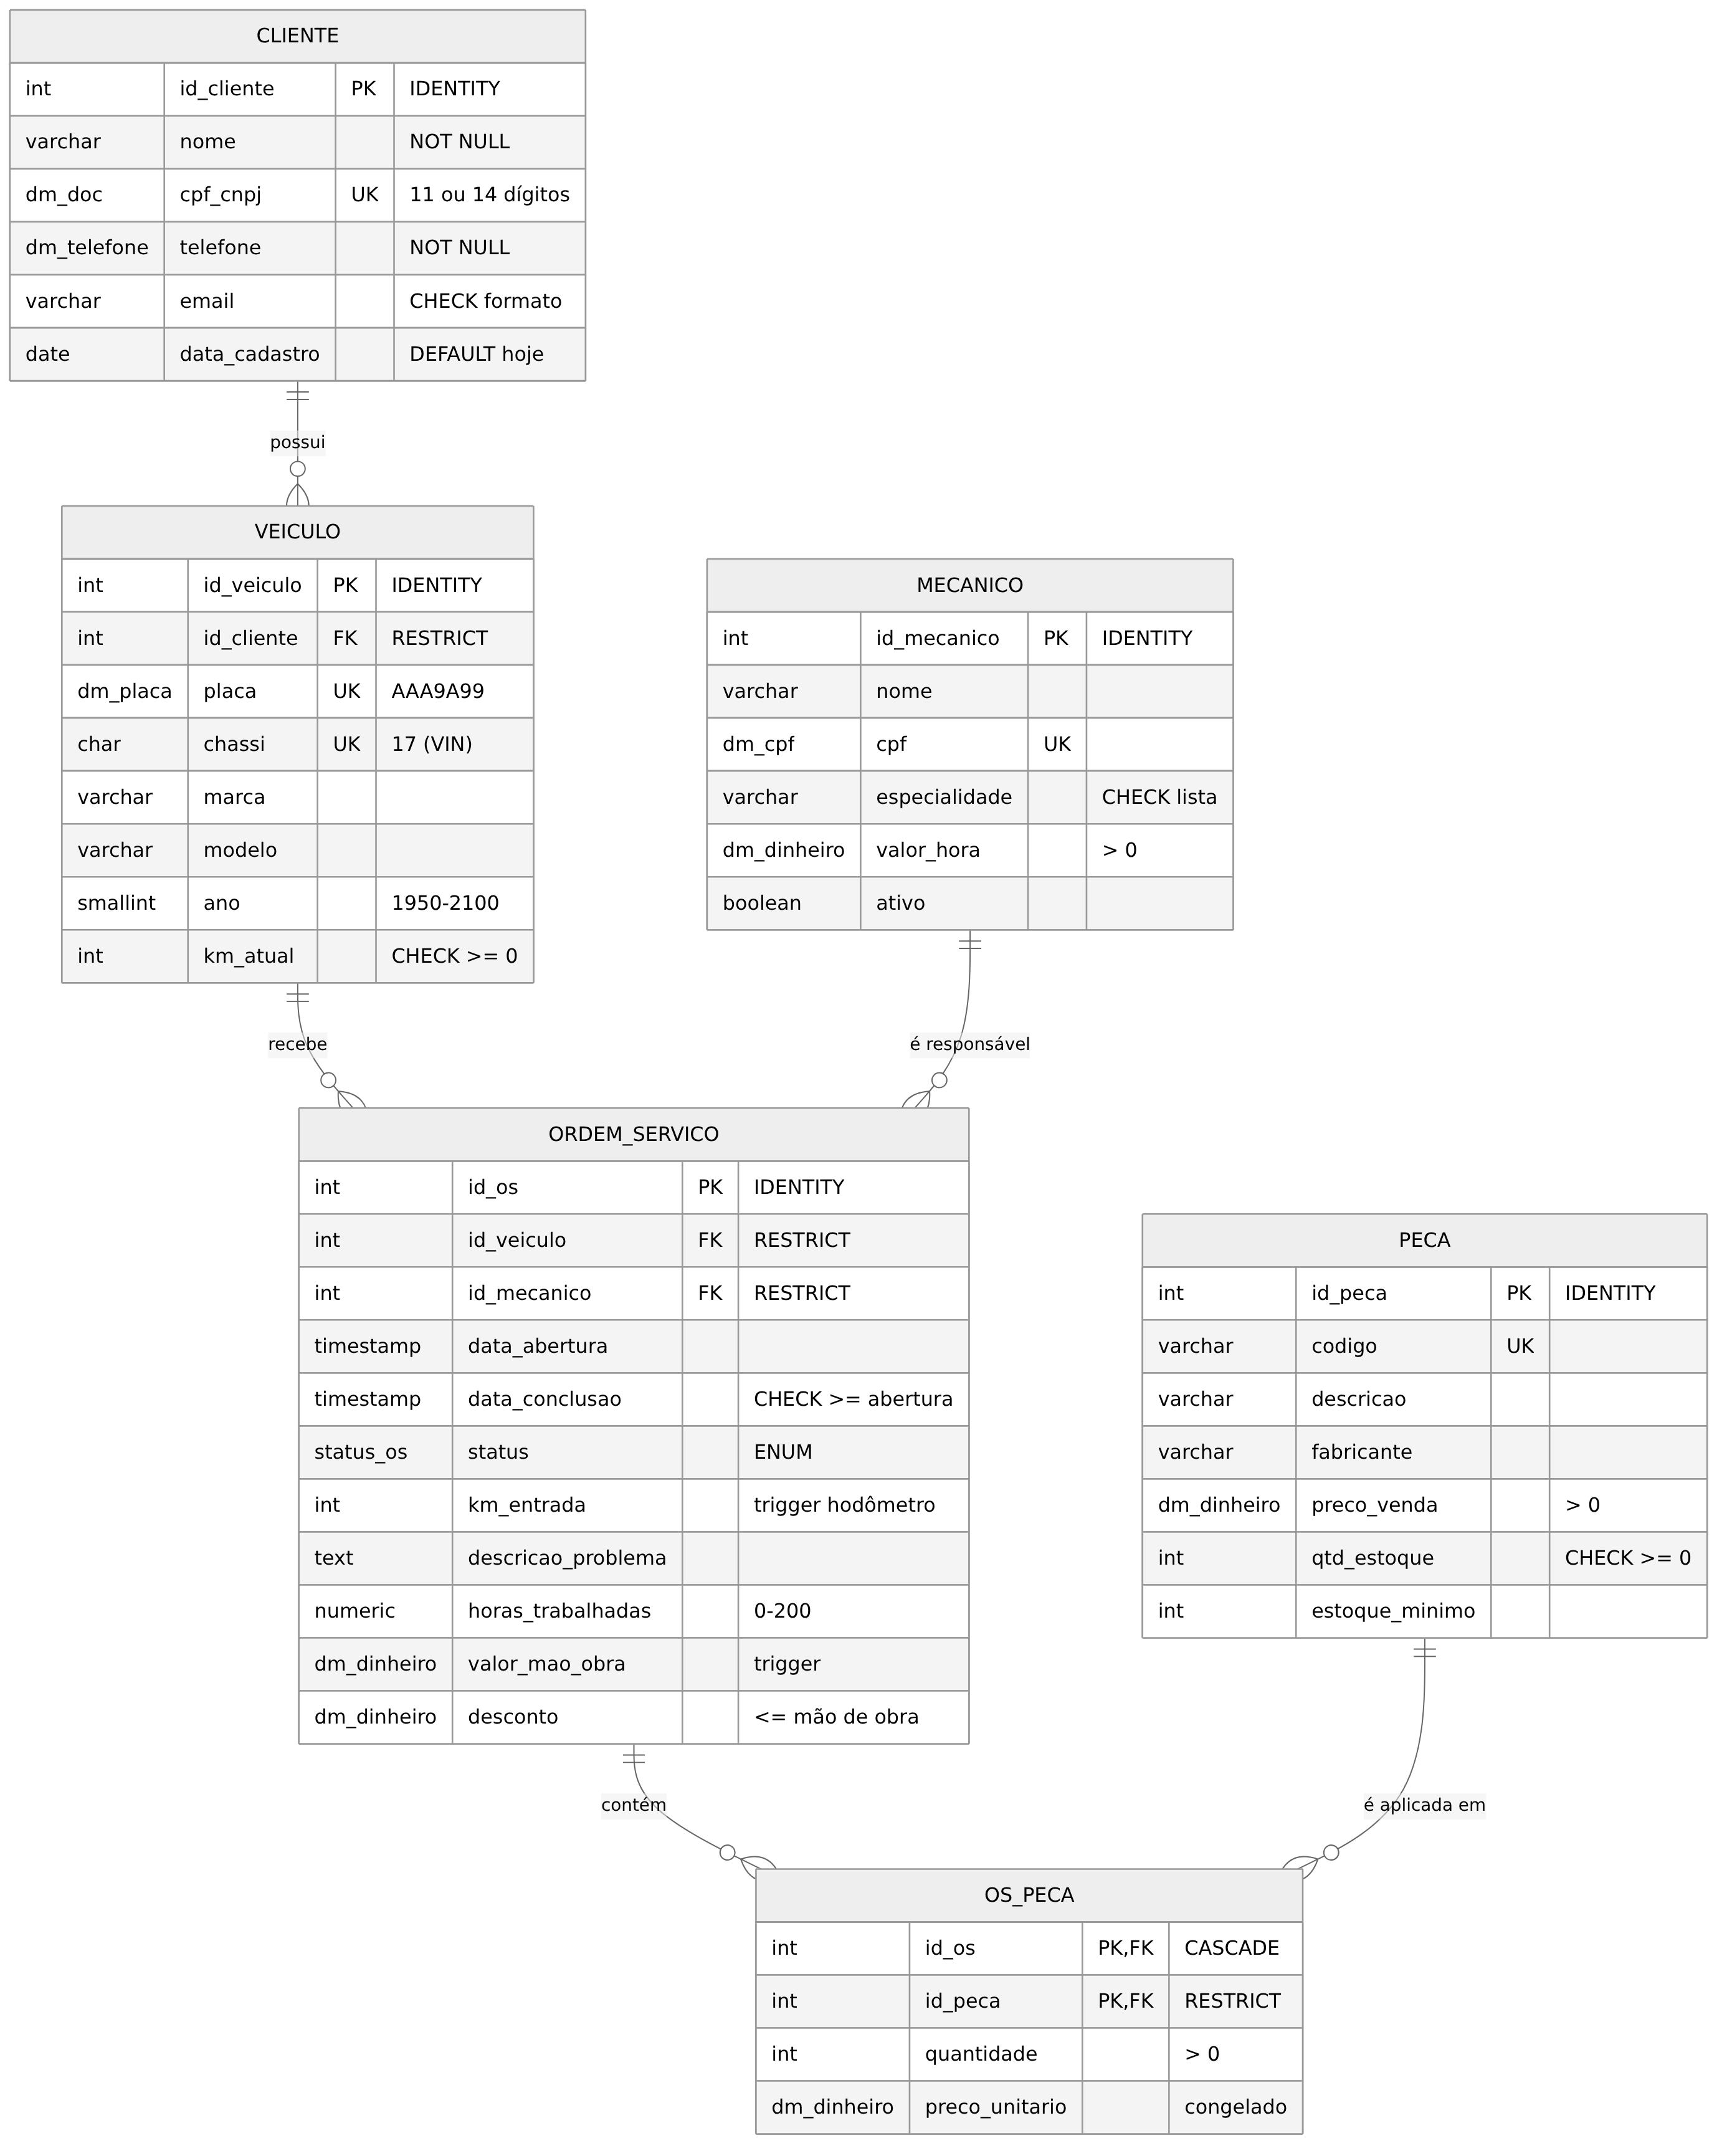
\includegraphics[width=.78\linewidth]{figuras/der.png}
  \caption{Diagrama entidade-relacionamento, com tipos e restrições de cada coluna.}
  \label{fig:der}
\end{figure}

A Figura~\ref{fig:arquitetura} mostra a arquitetura da solução. Os
usuários (recepção, mecânicos e gerência) acessam o \emph{schema}
\cod{oficina}, em que os domínios definem os formatos, as tabelas
garantem as restrições declarativas, os gatilhos aplicam as regras que
envolvem mais de uma tabela e a visão \cod{vw\_os\_total} calcula o
valor de cada OS. O repositório contém os scripts que criam o banco, os
testes, as medições e as evidências geradas.

\begin{figure}[!htbp]
  \centering
  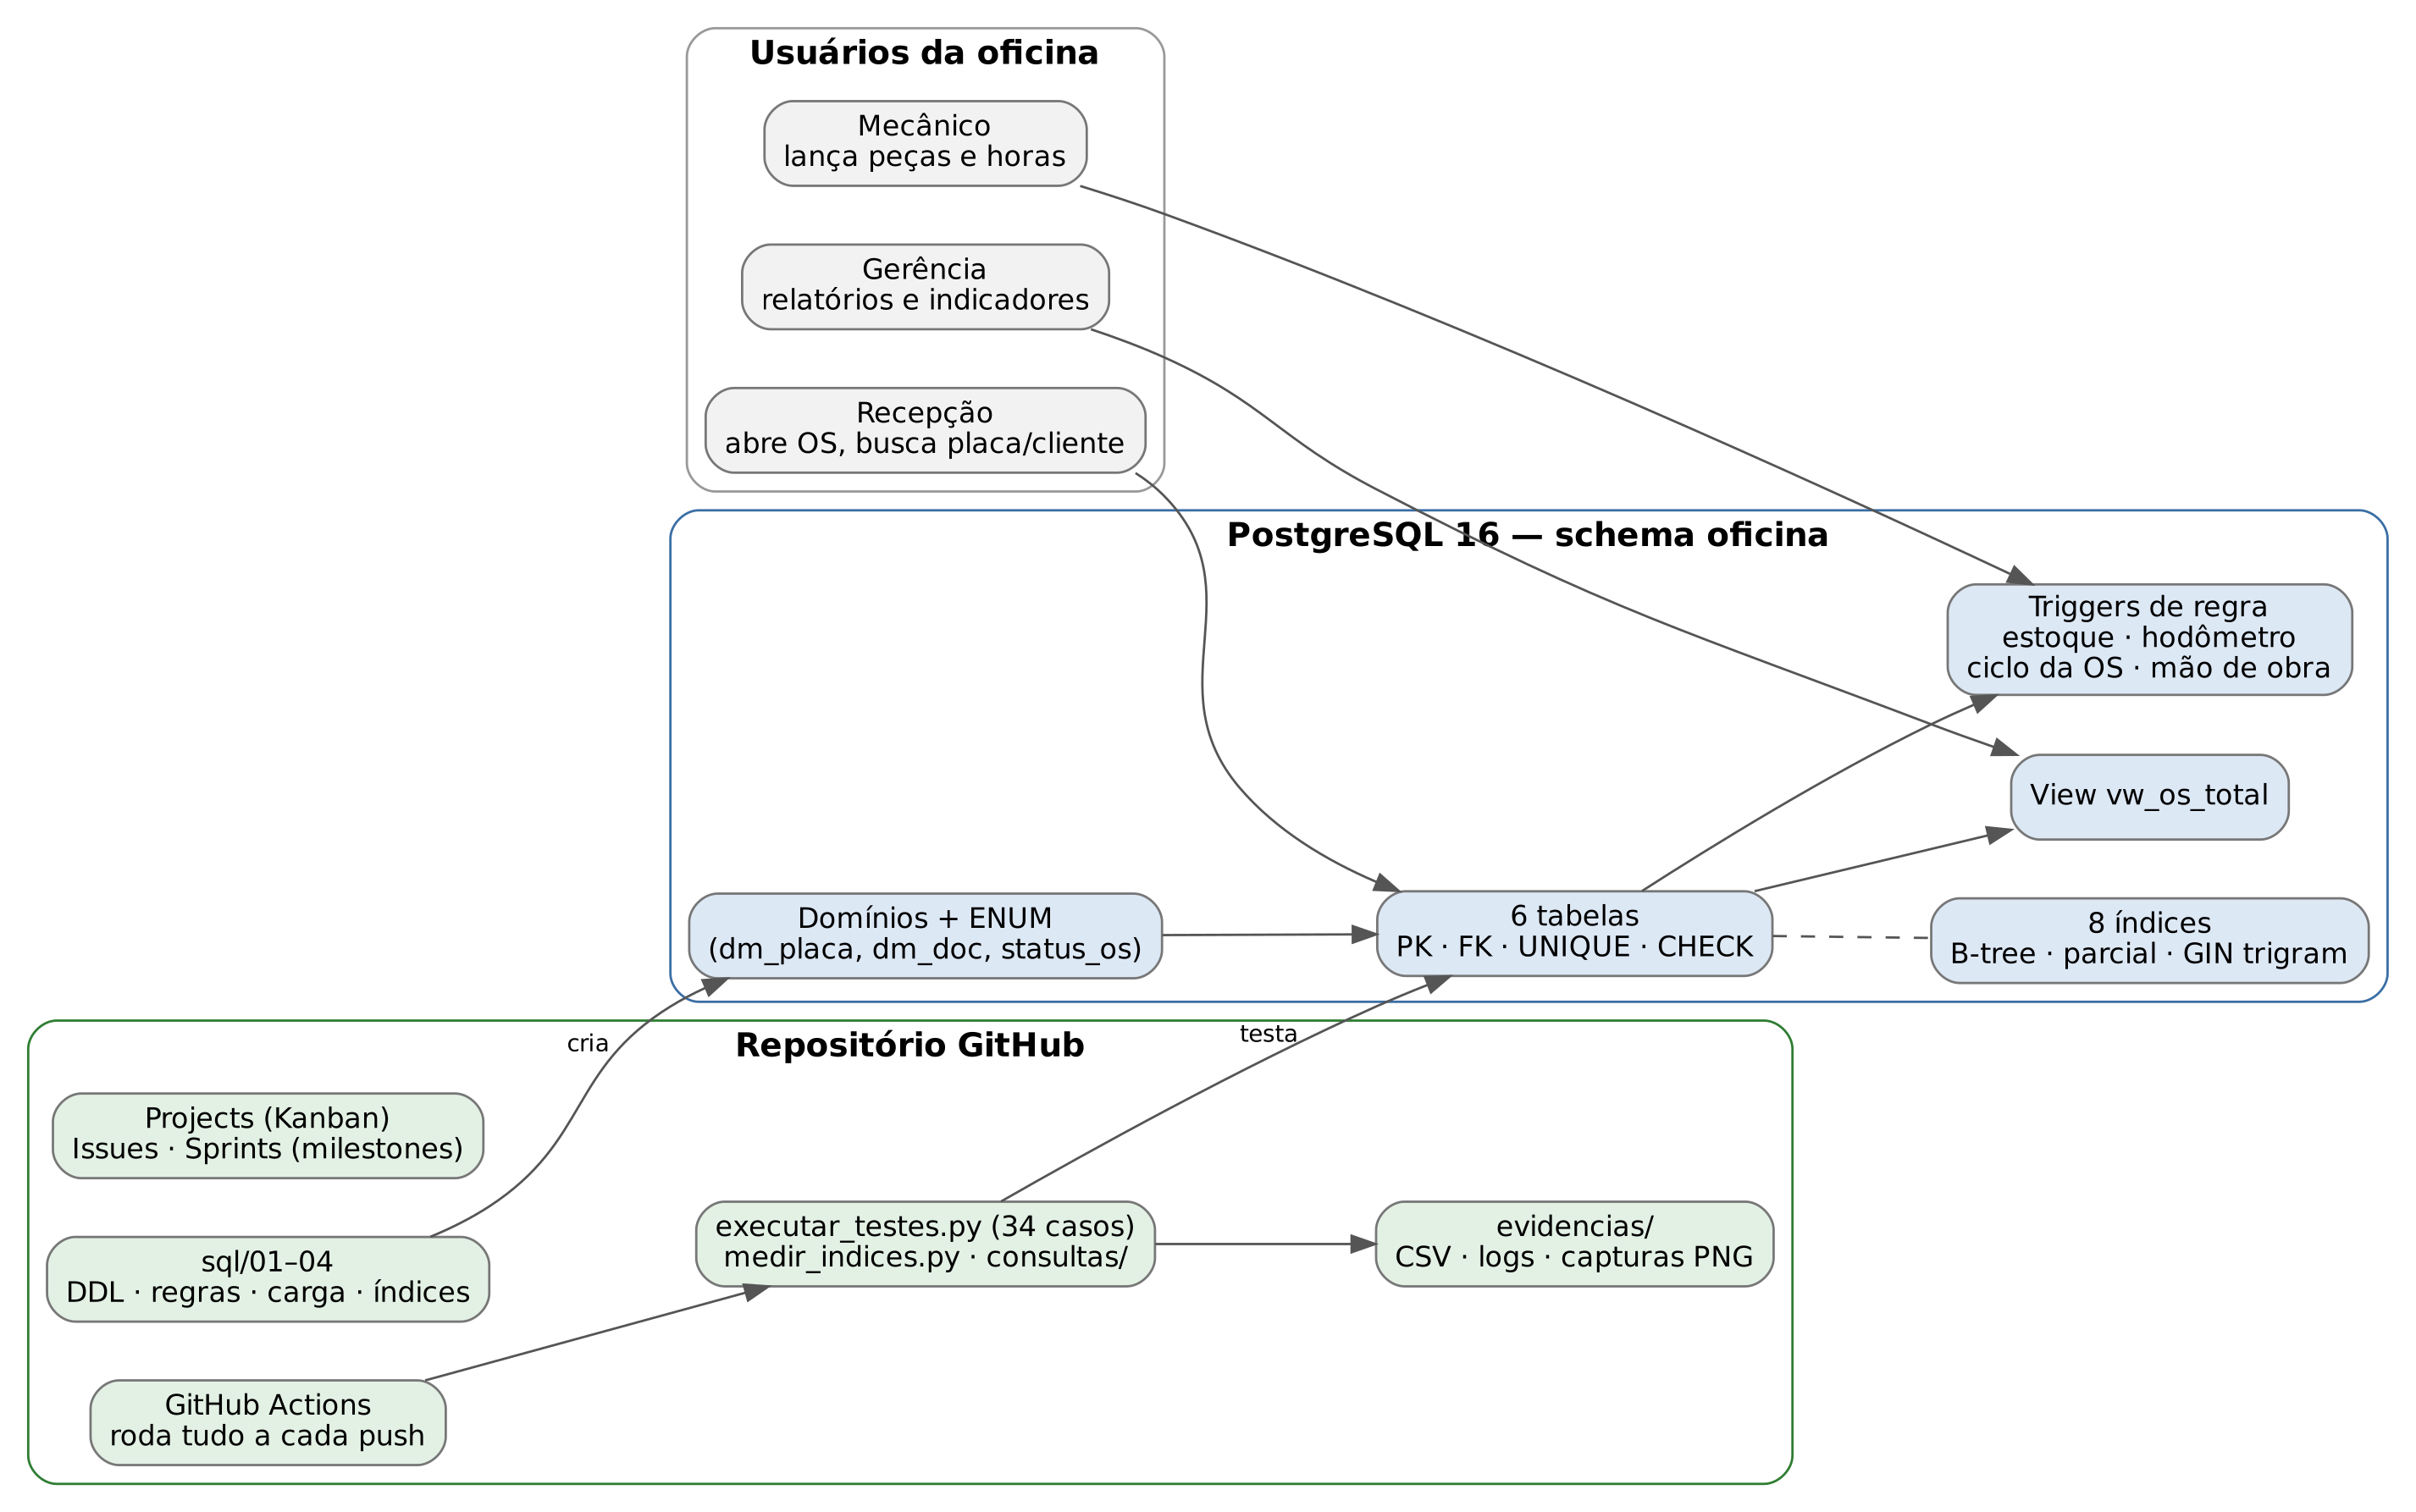
\includegraphics[width=\linewidth]{figuras/arquitetura.png}
  \caption{Arquitetura: usuários, banco de dados PostgreSQL e repositório GitHub com testes automatizados.}
  \label{fig:arquitetura}
\end{figure}

\subsection{Decisões de tipos de dados}

A Tabela~\ref{tab:tipos} resume as principais escolhas de tipo e o teste
que comprova cada uma. Dois pontos merecem destaque. Primeiro, valores
monetários usam \cod{NUMERIC(10,2)}, e não \cod{FLOAT}: o teste T07
(Figura~\ref{fig:t07}) mostra que, em ponto flutuante,
$0{,}1 + 0{,}2 = 0{,}30000000000000004$, enquanto em \cod{NUMERIC} o
resultado é exatamente $0{,}3$, e que 10,555 é arredondado para 10,56.
Segundo, regras de formato repetidas (placa, CPF/CNPJ, telefone,
dinheiro) foram centralizadas em domínios: a regra da placa é escrita
uma única vez e aceita tanto o padrão antigo (ABC1234) quanto o
Mercosul (RIO2A18).

\begin{table}[!htbp]
  \centering
  \caption{Principais decisões de tipos de dados e teste que as comprova.}
  \label{tab:tipos}
  \footnotesize\setlength{\tabcolsep}{4pt}\renewcommand{\cod}[1]{\texttt{#1}}
  \begin{tabular}{p{2.3cm}p{3.6cm}p{5.6cm}c}
    \hline
    Dado & Tipo escolhido & Justificativa & Teste \\ \hline
    Placa & domínio \cod{dm\_placa} (\cod{CHAR(7)} + regex) & tamanho fixo; aceita padrão antigo e Mercosul & T01--T03 \\
    Ano do veículo & \cod{SMALLINT} + \cod{CHECK} & 2 bytes bastam; texto e valores absurdos são rejeitados & T04, T05 \\
    Preço, mão de obra & \cod{NUMERIC(10,2)} & exato, sem erro de arredondamento binário & T06, T07 \\
    Status da OS & \cod{ENUM status\_os} & conjunto fechado de cinco estados; digitação livre bloqueada & T08 \\
    Datas da OS & \cod{TIMESTAMP} & registra hora de abertura e conclusão; datas inexistentes são rejeitadas & T09 \\
    CPF/CNPJ & domínio \cod{dm\_doc} & apenas 11 ou 14 dígitos, sem pontuação, para o \cod{UNIQUE} funcionar & T10, R02 \\
    Telefone & domínio \cod{dm\_telefone} & DDD + número, só dígitos & T11 \\ \hline
  \end{tabular}
\end{table}

\begin{figure}[!htbp]
  \centering
  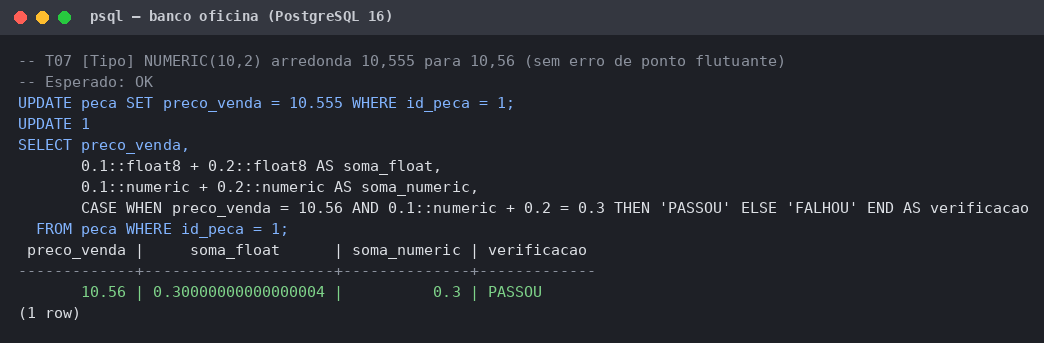
\includegraphics[width=.85\linewidth]{figuras/t07.png}
  \caption{Teste T07: \texttt{NUMERIC} é exato e arredonda para duas casas; \texttt{FLOAT} acumula erro.}
  \label{fig:t07}
\end{figure}

\subsection{Restrições e regras de negócio}

As restrições declarativas cobrem as regras que dependem só da própria
linha: \emph{UNIQUE} para placa, chassi e CPF/CNPJ; \emph{FOREIGN KEY}
com \emph{RESTRICT} para impedir a exclusão de um cliente que tem
veículos; \emph{CASCADE} de \cod{ordem\_servico} para \cod{os\_peca}; e
\emph{CHECK}s que relacionam colunas: a conclusão não pode ser anterior à
abertura, uma OS está \cod{CONCLUIDA} se e somente se tem data de
conclusão, e o desconto não pode superar a mão de obra.

As regras que envolvem outra tabela ou uma mudança de estado foram
implementadas em cinco gatilhos: (R1) o preço da peça é copiado do
catálogo quando não é informado; (R2) uma OS concluída ou cancelada não
aceita alteração de peças; (R3) lançar uma peça baixa o estoque, e
remover devolve; (R4) só um mecânico ativo pode assumir uma OS e o
hodômetro não pode ser menor que o último registrado; e (R5) uma OS
concluída ou cancelada não volta a ser aberta, o cancelamento devolve as
peças ao estoque e a mão de obra é calculada como horas trabalhadas
vezes o valor-hora do mecânico.

Uma decisão importante foi \emph{onde} bloquear o estoque negativo. Em
vez de testar o saldo dentro do gatilho, o gatilho apenas subtrai a
quantidade, e a restrição \cod{ck\_peca\_estoque\_nao\_negativo}
(\cod{CHECK (qtd\_estoque >= 0)}) rejeita o resultado. Assim, a regra
vale também para qualquer atualização manual do estoque, e não só para
lançamentos em OS. A Figura~\ref{fig:g02} mostra o teste G02: com uma
unidade em estoque, a tentativa de lançar três é rejeitada com o código
23514, e o banco informa a linha que teria ficado com saldo $-2$.

\begin{figure}[!htbp]
  \centering
  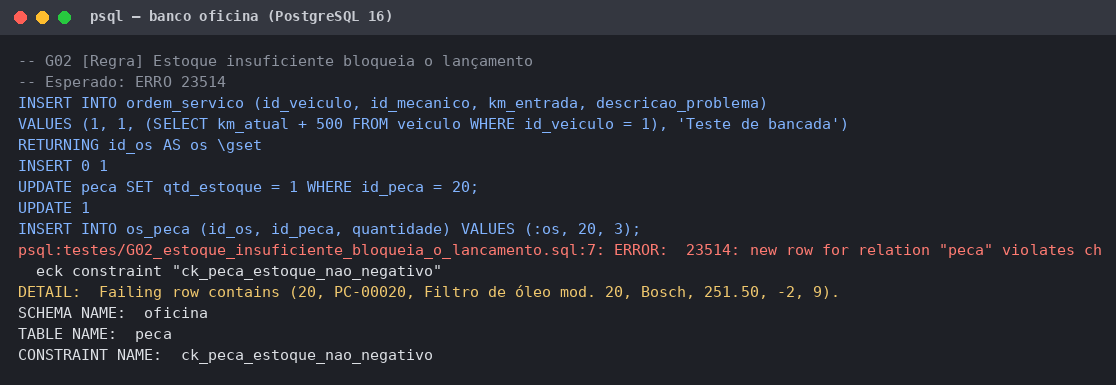
\includegraphics[width=\linewidth]{figuras/g02.png}
  \caption{Teste G02: estoque insuficiente. O gatilho subtrai e a restrição \texttt{CHECK} rejeita o saldo negativo.}
  \label{fig:g02}
\end{figure}

A Tabela~\ref{tab:testes} lista os 34 testes. Todos tiveram o resultado
esperado, e nos 26 casos de erro o código SQLSTATE devolvido foi
exatamente o previsto. A Figura~\ref{fig:g08} mostra um teste do tipo
``OK'': ao cancelar uma OS, as três unidades lançadas voltam ao estoque
(116 $\rightarrow$ 113 $\rightarrow$ 116). O teste G10 percorre o fluxo
completo (abrir, lançar duas peças, registrar 1,5 hora, aplicar desconto
de R\$~10,00 e concluir) e confere que a visão calcula
$245{,}90 + 112{,}50 - 10{,}00 = 348{,}40$.

{\footnotesize\setlength{\tabcolsep}{4pt}\renewcommand{\cod}[1]{\texttt{#1}}
\begin{longtable}{p{0.7cm}p{1.4cm}p{6.9cm}ll}
  \caption{Resultado dos 34 testes de tipos, restrições e regras (todos com o resultado esperado).}\label{tab:testes}\\
  \hline
  ID & Categoria & Teste & Esperado & Obtido \\ \hline
  \endfirsthead
  \hline
  ID & Categoria & Teste & Esperado & Obtido \\ \hline
  \endhead
  \hline
  \endfoot
  T01 & Tipo & Placa com 8 caracteres não cabe em CHAR(7) & ERRO 22001 & ERRO 22001 \\
  T02 & Tipo & Placa fora do padrão (domínio dm\_placa) & ERRO 23514 & ERRO 23514 \\
  T03 & Tipo & Placa Mercosul válida é aceita & OK & OK \\
  T04 & Tipo & Texto em coluna SMALLINT (ano) & ERRO 22P02 & ERRO 22P02 \\
  T05 & Tipo & Ano 40000 estoura o limite de SMALLINT & ERRO 22003 & ERRO 22003 \\
  T06 & Tipo & Valor acima de NUMERIC(10,2) é rejeitado & ERRO 22003 & ERRO 22003 \\
  T07 & Tipo & NUMERIC(10,2) arredonda 10,555 para 10,56 (sem erro de ponto flutuante) & OK & OK \\
  T08 & Tipo & Status fora do ENUM status\_os & ERRO 22P02 & ERRO 22P02 \\
  T09 & Tipo & Data inexistente (30/02) em TIMESTAMP & ERRO 22008 & ERRO 22008 \\
  T10 & Tipo & CPF com pontuação viola o domínio dm\_doc & ERRO 23514 & ERRO 23514 \\
  T11 & Tipo & Telefone com letras viola o domínio dm\_telefone & ERRO 23514 & ERRO 23514 \\
  R01 & Restrição & NOT NULL: cliente sem nome & ERRO 23502 & ERRO 23502 \\
  R02 & Restrição & UNIQUE: CPF/CNPJ repetido & ERRO 23505 & ERRO 23505 \\
  R03 & Restrição & UNIQUE: placa repetida & ERRO 23505 & ERRO 23505 \\
  R04 & Restrição & FOREIGN KEY: veículo de cliente inexistente & ERRO 23503 & ERRO 23503 \\
  R05 & Restrição & ON DELETE RESTRICT: excluir cliente que tem veículos & ERRO 23503 & ERRO 23503 \\
  R06 & Restrição & CHECK: km do veículo negativo & ERRO 23514 & ERRO 23514 \\
  R07 & Restrição & CHECK: conclusão antes da abertura & ERRO 23514 & ERRO 23514 \\
  R08 & Restrição & CHECK: OS CONCLUIDA sem data de conclusão & ERRO 23514 & ERRO 23514 \\
  R09 & Restrição & CHECK: desconto maior que a mão de obra & ERRO 23514 & ERRO 23514 \\
  R10 & Restrição & PRIMARY KEY composta: mesma peça duas vezes na OS & ERRO 23505 & ERRO 23505 \\
  R11 & Restrição & CHECK: quantidade zero de peça & ERRO 23514 & ERRO 23514 \\
  R12 & Restrição & CHECK: e-mail sem @ & ERRO 23514 & ERRO 23514 \\
  R13 & Restrição & ON DELETE CASCADE: excluir OS aberta remove seus itens & OK & OK \\
  G01 & Regra & Lançar peça na OS baixa o estoque automaticamente & OK & OK \\
  G02 & Regra & Estoque insuficiente bloqueia o lançamento & ERRO 23514 & ERRO 23514 \\
  G03 & Regra & Preço da peça é copiado do catálogo quando omitido & OK & OK \\
  G04 & Regra & OS CONCLUIDA não aceita novas peças & ERRO P0001 & ERRO P0001 \\
  G05 & Regra & Mecânico inativo não pode assumir OS & ERRO P0001 & ERRO P0001 \\
  G06 & Regra & Hodômetro não pode voltar (km\_entrada < km\_atual) & ERRO P0001 & ERRO P0001 \\
  G07 & Regra & OS CONCLUIDA não pode ser reaberta & ERRO P0001 & ERRO P0001 \\
  G08 & Regra & Cancelar a OS devolve as peças ao estoque & OK & OK \\
  G09 & Regra & Mão de obra = horas trabalhadas x valor/hora do mecânico & OK & OK \\
  G10 & Regra & Fluxo completo: abrir, lançar peças, concluir e faturar & OK & OK \\
\end{longtable}
}

\begin{figure}[!htbp]
  \centering
  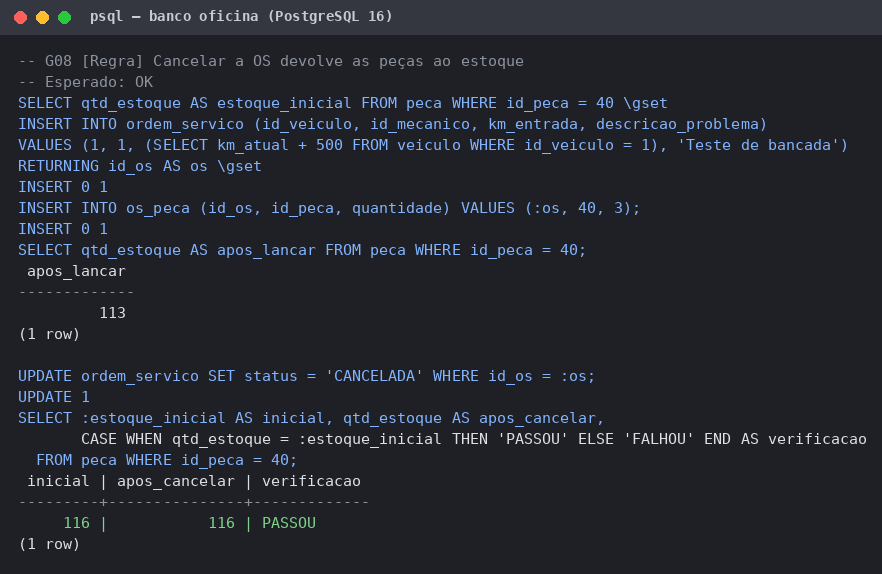
\includegraphics[width=.8\linewidth]{figuras/g08.png}
  \caption{Teste G08: o cancelamento da OS devolve as peças ao estoque.}
  \label{fig:g08}
\end{figure}

\subsection{Índices}

Cada índice foi criado para atender a uma consulta da rotina da oficina.
A Tabela~\ref{tab:indices} mostra o resultado das medições. Antes dos
índices, quase todas as consultas faziam leitura sequencial
(\emph{Seq Scan}) das 8.204 páginas da tabela \cod{ordem\_servico}
(cerca de 64~MB).

\begin{table}[!htbp]
  \centering
  \caption{Efeito dos índices (mediana de 7 execuções de \texttt{EXPLAIN ANALYZE}; 300 mil OS).}
  \label{tab:indices}
  \footnotesize\setlength{\tabcolsep}{4pt}\renewcommand{\cod}[1]{\texttt{#1}}
  \begin{tabular}{p{4.1cm}p{3.6cm}rrr}
    \hline
    Consulta & Índice & Antes (ms) & Depois (ms) & Páginas lidas \\ \hline
    B1 Histórico por placa & \cod{(id\_veiculo, data\_abertura DESC)} & 30,60 & 0,25 & 8.323 $\rightarrow$ 31 \\
    B2 Painel de OS pendentes & parcial em \cod{data\_abertura} & 24,80 & 0,35 & 8.276 $\rightarrow$ 52 \\
    B3 Produção do mecânico no mês & \cod{(id\_mecanico, data\_abertura)} & 24,32 & 0,84 & 8.204 $\rightarrow$ 200 \\
    B4 Faturamento do mês & \cod{(data\_conclusao)} & 23,52 & 6,28 & 8.204 $\rightarrow$ 2.590 \\
    B5 Consumo de uma peça & \cod{os\_peca (id\_peca)} & 29,25 & 2,56 & 2.870 $\rightarrow$ 611 \\
    B6 Veículos de um cliente & \cod{veiculo (id\_cliente)} & 2,00 & 0,14 & 613 $\rightarrow$ 4 \\
    B7 Cliente por parte do nome & GIN \cod{pg\_trgm} & 12,04 & 0,97 & 266 $\rightarrow$ 174 \\
    B8 OS concluídas (95\% das linhas) & \cod{(status)} & 46,32 & 49,09 & ignorado \\
    B9 OS abertas (0,2\% das linhas) & \cod{(status)} & 25,46 & 1,59 & 8.204 $\rightarrow$ 532 \\ \hline
    W1 Inserir 20 mil OS & todos os 8 & 1.250 & 1.578 & +26\% \\ \hline
  \end{tabular}
\end{table}

O maior ganho veio do índice composto do histórico por placa (B1): a
busca da placa já usava o índice criado pelo \emph{UNIQUE}, mas as OS
do veículo exigiam ler a tabela inteira. Com o índice
\cod{(id\_veiculo, data\_abertura DESC)}, o banco encontra as OS já na
ordem pedida e lê 31 páginas em vez de 8.323
(Figura~\ref{fig:planos}). O painel de pendências (B2) usa um índice
\emph{parcial}, que contém apenas as cerca de 2.800 OS não finalizadas:
ocupa 464~kB, contra cerca de 7~MB de um índice comum de data sobre a
tabela inteira (\cod{ix\_os\_conclusao}), e continua pequeno à medida que o histórico cresce.

\begin{figure}[!htbp]
  \centering
  \begin{minipage}[t]{0.49\linewidth}\centering
    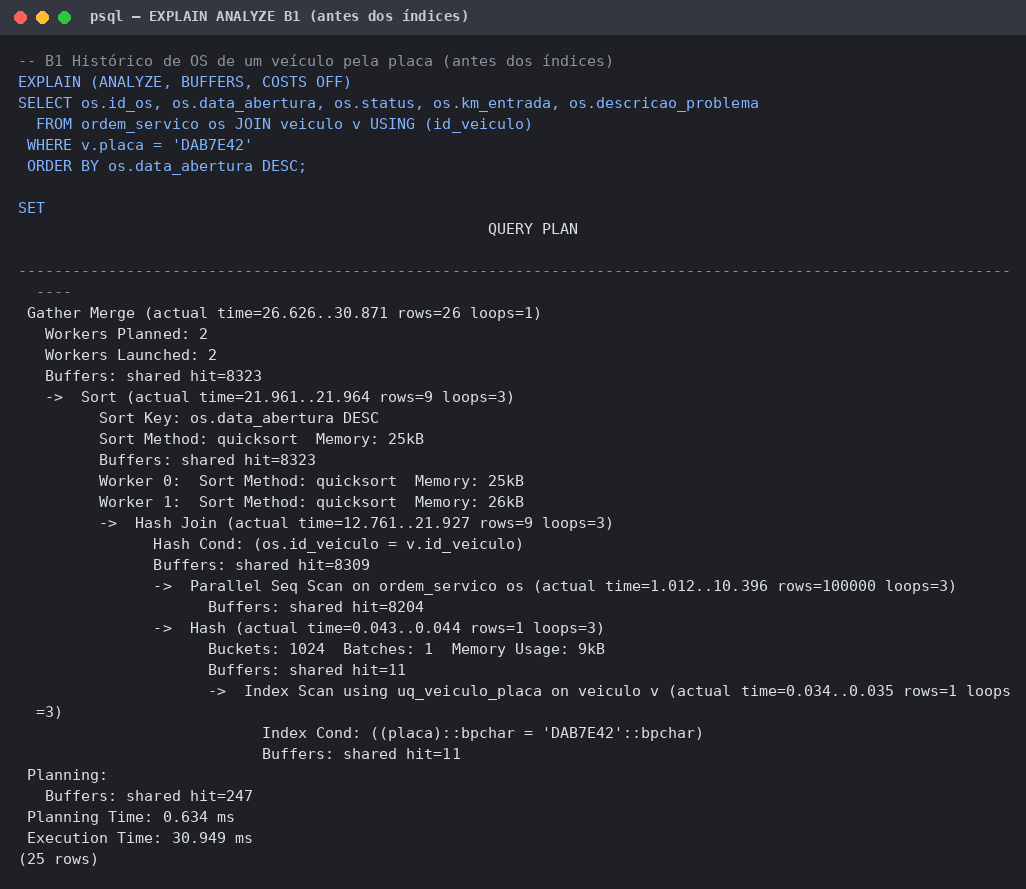
\includegraphics[width=\linewidth]{figuras/plano_B1_antes.png}\\
    {\footnotesize (a) antes: \emph{Seq Scan}, 8.323 páginas}
  \end{minipage}\hfill
  \begin{minipage}[t]{0.49\linewidth}\centering
    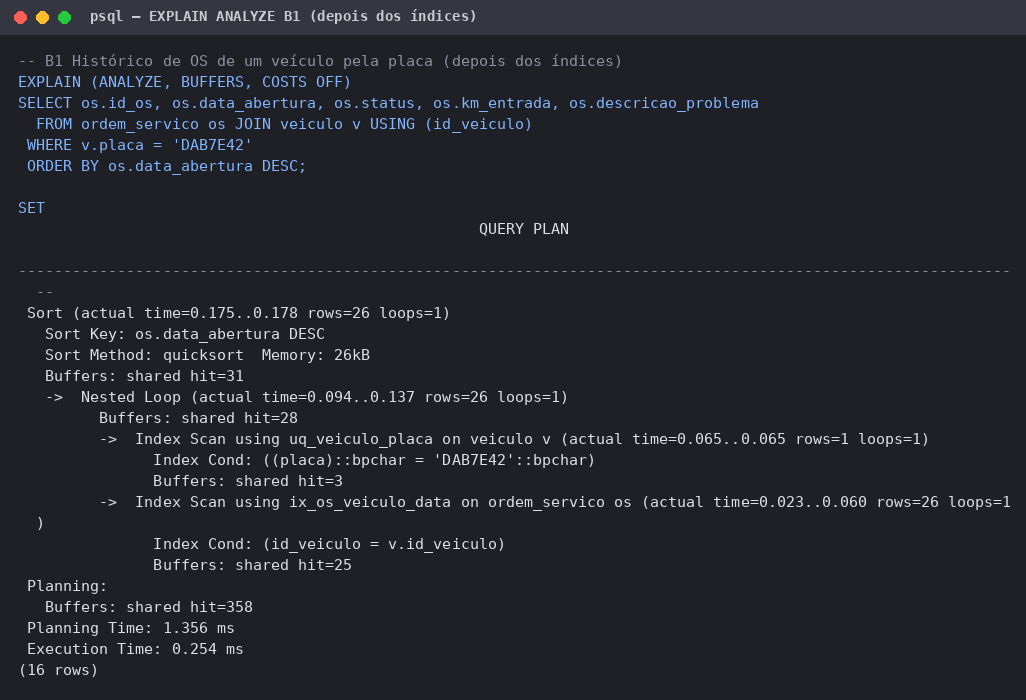
\includegraphics[width=\linewidth]{figuras/plano_B1_depois.png}\\
    {\footnotesize (b) depois: \emph{Index Scan}, 31 páginas}
  \end{minipage}
  \caption{Plano de execução da consulta B1 (histórico por placa) antes e depois do índice.}
  \label{fig:planos}
\end{figure}

Três resultados contrariam a ideia de que ``índice sempre ajuda'' e
justificam testar em vez de supor:

\begin{itemize}
  \item \textbf{Baixa seletividade (B8 x B9).} O mesmo índice em
  \cod{status} foi \emph{ignorado} pelo otimizador quando o filtro
  pegava 95\% das linhas (\cod{CONCLUIDA}), porque ler a tabela em
  sequência é mais barato que saltar entre índice e tabela, e foi usado
  quando o filtro pegava 0,2\% (\cod{ABERTA}). Como o índice parcial
  I2 já atende às OS pendentes, o índice em \cod{status} é candidato a
  remoção.
  \item \textbf{Ganho moderado no faturamento (B4).} As OS de um mês
  estão espalhadas fisicamente pela tabela, pois a carga não seguiu a
  ordem cronológica; o índice localiza as 4 mil linhas, mas ainda é
  preciso visitar 2.590 páginas. O ganho foi de 3,7 vezes, bem menor que
  o das demais consultas.
  \item \textbf{Custo na escrita (W1).} Com os oito índices, inserir
  20 mil OS ficou 26\% mais lento, e os índices ocupam cerca de 40~MB.
  Para uma oficina, em que as consultas são muito mais frequentes que as
  inserções, a troca compensa, mas ela existe e foi medida.
\end{itemize}

\subsection{Visão de totais: \emph{GROUP BY} x \emph{LATERAL}}

A primeira versão da visão \cod{vw\_os\_total} somava as peças em uma
subconsulta com \emph{GROUP BY}. O teste da consulta C01 (histórico por
placa usando a visão) revelou que essa forma agrupava os 450 mil itens
antes de aplicar o filtro da placa. A segunda versão usa
\cod{CROSS JOIN LATERAL}, que soma as peças de cada OS somente depois
do filtro. A Tabela~\ref{tab:view} mostra que não há versão melhor em
todos os casos: a nova é 633 vezes mais rápida para uma placa, mas duas
vezes mais lenta para o relatório que soma todas as OS. A decisão foi
manter a versão \emph{LATERAL} na visão, usada no balcão, e escrever os
relatórios gerais (como o ranking de clientes, C06) com agregação direta
nas tabelas.

\begin{table}[!htbp]
  \centering
  \caption{Tempo da visão de totais nas duas versões (mediana de 7 execuções).}
  \label{tab:view}
  \footnotesize
  \begin{tabular}{lrrr}
    \hline
    Consulta & v1 \emph{GROUP BY} (ms) & v2 \emph{LATERAL} (ms) & v1/v2 \\ \hline
    Histórico de uma placa & 314,46 & 0,50 & 632,7 \\
    Faturamento de set/2026 & 343,51 & 68,57 & 5,0 \\
    Faturamento total (todas as OS) & 969,21 & 2.114,03 & 0,5 \\ \hline
  \end{tabular}
\end{table}

\subsection{Consultas de negócio}

Oito consultas respondem às perguntas da oficina (pasta
\cod{consultas/}): histórico por placa (C01); faturamento mensal com
peças, mão de obra e tíquete médio (C02); ranking de mecânicos com
\cod{RANK()} (C03); peças abaixo do estoque mínimo, com o consumo dos
últimos 90 dias (C04); OS pendentes há mais de sete dias (C05); os dez
clientes que mais gastaram e sua participação no faturamento (C06);
taxa de retrabalho por mecânico (C07); e uma conferência de totais
(C08). Em 2026, o tíquete médio mensal ficou entre R\$~748 e R\$~770.
A consulta C08 confirmou que o total das OS concluídas calculado pela
visão é igual à soma feita direto nas tabelas (R\$~216.799.627,25 nos
dois casos).

O teste da C04 encontrou um erro na primeira versão da consulta: a
junção externa com a condição de data no \emph{ON} somava o consumo de
\emph{todos} os períodos, e algumas peças apareciam com cerca de 3.000
unidades consumidas em 90 dias. Após mover a agregação para uma
subconsulta filtrada, o maior consumo passou a ser de 61 unidades,
coerente com o volume de OS. A Figura~\ref{fig:c07} mostra a C07, que usa
a função de janela \cod{LAG()} para comparar cada OS com a anterior do
mesmo veículo: quando o carro volta com o mesmo problema em até 30 dias,
o retorno é atribuído ao mecânico da OS anterior. A taxa mais alta foi
de 1,85\%.

\begin{figure}[!htbp]
  \centering
  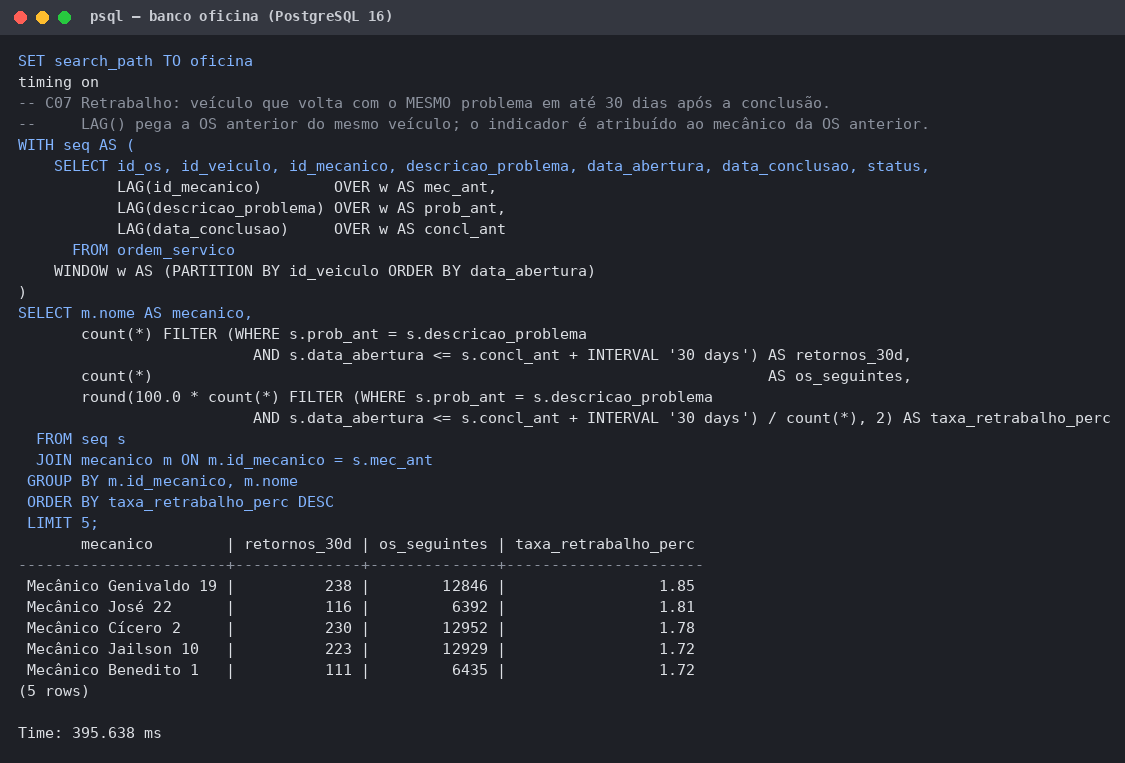
\includegraphics[width=\linewidth]{figuras/c07.png}
  \caption{Consulta C07: taxa de retrabalho por mecânico calculada com a função de janela \texttt{LAG()}.}
  \label{fig:c07}
\end{figure}

\subsection{Acompanhamento ágil no GitHub}

O repositório reúne o SQL (\cod{sql/01} a \cod{sql/04}), os 34 testes,
as consultas, os scripts e a pasta \cod{evidencias/}, com um arquivo de
log, uma captura de tela por teste e as tabelas em CSV. O script
\cod{criar\_quadro\_github.sh} cria os rótulos, as cinco sprints como
\emph{milestones}, 17 \emph{issues} de backlog e o quadro Kanban no
GitHub Projects, em que o professor acompanha o que está a fazer, em
andamento e concluído. O GitHub Actions recria o banco e executa todos
os testes a cada envio, de modo que o selo ``passing'' no README é ele
próprio uma evidência atualizada.

% =====================================================================
\section{Conclusão}

Este trabalho implementou em PostgreSQL um banco de dados para o
controle de ordens de serviço de uma oficina mecânica e verificou cada
decisão por teste. As seis falhas descritas na introdução (placa
duplicada, peça sem baixa, OS sem responsável, hodômetro voltando, OS
fechada alterada e histórico lento) passaram a ser impedidas ou
resolvidas pelo próprio banco, conforme comprovado pelos 34 testes, todos
com o resultado e o código de erro esperados. Os índices reduziram as
consultas da rotina em uma a duas ordens de grandeza, e o histórico por
placa caiu de 30,60~ms para 0,25~ms.

A principal lição veio dos resultados negativos: um índice ignorado por
baixa seletividade, uma visão mais rápida em um caso e mais lenta em
outro, um custo de 26\% na escrita e um erro de lógica encontrado em
uma consulta de estoque. Nenhum deles teria aparecido sem teste.

Como limitações, os dados são sintéticos e as medições foram feitas em
uma única máquina, então os tempos absolutos variam; o número de páginas
lidas é a medida mais estável. O CPF é validado apenas no formato, sem
cálculo dos dígitos verificadores, e o comportamento do estoque com
vários mecânicos lançando a mesma peça ao mesmo tempo não foi testado.
Como trabalhos futuros, sugere-se validar os dígitos do CPF/CNPJ,
testar a concorrência no estoque com duas sessões simultâneas, avaliar o
reagrupamento físico da tabela por data (\cod{CLUSTER}) para o
faturamento mensal e testar o modelo com dados reais anonimizados de uma
oficina de Aracaju.

% =====================================================================
\section*{Declaração de Uso de Inteligência Artificial}

Em conformidade com a Portaria CNPq nº 2.664/2026 e o Art. 12º do
Manual de Normas, os autores declaram que utilizaram a ferramenta de IA
generativa Claude (Anthropic, modelo Claude Opus 5.5) nas seguintes
etapas: (i) apoio à modelagem e à escrita do código SQL (tabelas,
restrições, gatilhos, índices e consultas); (ii) escrita dos scripts de
automação dos testes e das medições; e (iii) redação preliminar e
revisão do texto deste artigo. Todos os testes e medições foram
executados no PostgreSQL, e os números apresentados foram extraídos das
saídas reais do banco, disponíveis na pasta \cod{evidencias/} do
repositório. Os autores revisaram o código, reexecutaram os testes e são
integralmente responsáveis pelo conteúdo. [Revisar e ajustar esta
declaração conforme o uso efetivo pelo grupo.]

\begin{thebibliography}{9}

\bibitem{codd1970}
Codd, E. F.
\newblock A relational model of data for large shared data banks.
\newblock \emph{Communications of the ACM}, v. 13, n. 6, p. 377--387, 1970.

\bibitem{elmasri2016}
Elmasri, R.; Navathe, S. B.
\newblock \emph{Fundamentals of Database Systems}. 7. ed. Boston: Pearson, 2016.

\bibitem{silberschatz2019}
Silberschatz, A.; Korth, H. F.; Sudarshan, S.
\newblock \emph{Database System Concepts}. 7. ed. New York: McGraw-Hill, 2019.

\bibitem{pgdocs}
PostgreSQL Global Development Group.
\newblock \emph{PostgreSQL 16 Documentation}: Constraints; Domains;
Triggers; Indexes; Partial Indexes; Using EXPLAIN; pg\_trgm.
\newblock Disponível em: \url{https://www.postgresql.org/docs/16/}. Acesso em: 26 out. 2026.

\bibitem{winand2012}
Winand, M.
\newblock \emph{SQL Performance Explained}. Viena: Markus Winand, 2012.

\bibitem{scrum2020}
Schwaber, K.; Sutherland, J.
\newblock \emph{The Scrum Guide}. 2020.
\newblock Disponível em: \url{https://scrumguides.org}. Acesso em: 26 out. 2026.

\end{thebibliography}

\end{document}
